\documentclass{article}\usepackage[]{graphicx}\usepackage[]{color}
% maxwidth is the original width if it is less than linewidth
% otherwise use linewidth (to make sure the graphics do not exceed the margin)
\makeatletter
\def\maxwidth{ %
  \ifdim\Gin@nat@width>\linewidth
    \linewidth
  \else
    \Gin@nat@width
  \fi
}
\makeatother

\definecolor{fgcolor}{rgb}{0.345, 0.345, 0.345}
\newcommand{\hlnum}[1]{\textcolor[rgb]{0.686,0.059,0.569}{#1}}%
\newcommand{\hlstr}[1]{\textcolor[rgb]{0.192,0.494,0.8}{#1}}%
\newcommand{\hlcom}[1]{\textcolor[rgb]{0.678,0.584,0.686}{\textit{#1}}}%
\newcommand{\hlopt}[1]{\textcolor[rgb]{0,0,0}{#1}}%
\newcommand{\hlstd}[1]{\textcolor[rgb]{0.345,0.345,0.345}{#1}}%
\newcommand{\hlkwa}[1]{\textcolor[rgb]{0.161,0.373,0.58}{\textbf{#1}}}%
\newcommand{\hlkwb}[1]{\textcolor[rgb]{0.69,0.353,0.396}{#1}}%
\newcommand{\hlkwc}[1]{\textcolor[rgb]{0.333,0.667,0.333}{#1}}%
\newcommand{\hlkwd}[1]{\textcolor[rgb]{0.737,0.353,0.396}{\textbf{#1}}}%
\let\hlipl\hlkwb

\usepackage{framed}
\makeatletter
\newenvironment{kframe}{%
 \def\at@end@of@kframe{}%
 \ifinner\ifhmode%
  \def\at@end@of@kframe{\end{minipage}}%
  \begin{minipage}{\columnwidth}%
 \fi\fi%
 \def\FrameCommand##1{\hskip\@totalleftmargin \hskip-\fboxsep
 \colorbox{shadecolor}{##1}\hskip-\fboxsep
     % There is no \\@totalrightmargin, so:
     \hskip-\linewidth \hskip-\@totalleftmargin \hskip\columnwidth}%
 \MakeFramed {\advance\hsize-\width
   \@totalleftmargin\z@ \linewidth\hsize
   \@setminipage}}%
 {\par\unskip\endMakeFramed%
 \at@end@of@kframe}
\makeatother

\definecolor{shadecolor}{rgb}{.97, .97, .97}
\definecolor{messagecolor}{rgb}{0, 0, 0}
\definecolor{warningcolor}{rgb}{1, 0, 1}
\definecolor{errorcolor}{rgb}{1, 0, 0}
\newenvironment{knitrout}{}{} % an empty environment to be redefined in TeX

\usepackage{alltt}
\usepackage[margin = 1in]{geometry}
\usepackage{amsmath}
\usepackage{parskip}
\usepackage{url}
\title{ATUS Microdata Forecasting (Example for Portfolio)}
\author{Charles Ye}
\date{}
\IfFileExists{upquote.sty}{\usepackage{upquote}}{}
\begin{document}
\maketitle

\begin{knitrout}
\definecolor{shadecolor}{rgb}{0.969, 0.969, 0.969}\color{fgcolor}\begin{kframe}
\begin{alltt}
    \hlkwd{library}\hlstd{(tidyverse)}
    \hlkwd{library}\hlstd{(xtable)}
    \hlkwd{library}\hlstd{(glmnet)} \hlcom{# Elastic Net}
    \hlkwd{library}\hlstd{(e1071)} \hlcom{# SVM}

    \hlcom{# Settings for PDF compilation}
    \hlstd{knitr}\hlopt{::}\hlstd{opts_chunk}\hlopt{$}\hlkwd{set}\hlstd{(}
      \hlkwc{echo} \hlstd{= T,} \hlkwc{results} \hlstd{=} \hlstr{'asis'}\hlstd{,}
      \hlkwc{fig.width} \hlstd{=} \hlnum{10}\hlstd{,} \hlkwc{fig.height} \hlstd{=} \hlnum{4}\hlstd{,} \hlkwc{out.width} \hlstd{=} \hlstr{'5in'}\hlstd{,} \hlkwc{out.height} \hlstd{=} \hlstr{'2in'}\hlstd{,}
      \hlkwc{fig.pos} \hlstd{=} \hlstr{'!h'}\hlstd{,} \hlkwc{fig.align} \hlstd{=} \hlstr{'center'}\hlstd{,} \hlkwc{warnings} \hlstd{= F,} \hlkwc{message} \hlstd{= F}
      \hlstd{)}
    \hlkwd{options}\hlstd{(}\hlkwc{xtable.include.rownames} \hlstd{= F)}
    \hlkwd{options}\hlstd{(}\hlkwc{xtable.size} \hlstd{=} \hlstr{'footnotesize'}\hlstd{)}
    \hlkwd{options}\hlstd{(}\hlkwc{xtable.table.placement} \hlstd{=} \hlstr{'!h'}\hlstd{)}
\end{alltt}
\end{kframe}
\end{knitrout}

\section{Elastic Net Estimation}
We use a microdata dataset compiled from the American Time Use Survey (ATUS), see \url{https://www.bls.gov/tus/}.
\begin{kframe}
\begin{alltt}
  \hlcom{## Load Data from ATUS}
  \hlstd{tmp} \hlkwb{=} \hlkwd{tempfile}\hlstd{()}
  \hlkwd{download.file}\hlstd{(}\hlstr{'https://www.bls.gov/tus/special.requests/atusresp-2019.zip'}\hlstd{, tmp)}
  \hlstd{df1} \hlkwb{=} \hlkwd{unz}\hlstd{(tmp,} \hlstr{'atusresp_2019.dat'}\hlstd{)} \hlopt \hlstd{readr}\hlopt{::}\hlkwd{read_delim}\hlstd{(.,} \hlkwc{delim} \hlstd{=} \hlstr{','}\hlstd{)}
  \hlkwd{download.file}\hlstd{(}\hlstr{'https://www.bls.gov/tus/special.requests/atussum-2019.zip'}\hlstd{, tmp)}
  \hlstd{df2} \hlkwb{=} \hlkwd{unz}\hlstd{(tmp,} \hlstr{'atussum_2019.dat'}\hlstd{)} \hlopt \hlstd{readr}\hlopt{::}\hlkwd{read_delim}\hlstd{(.,} \hlkwc{delim} \hlstd{=} \hlstr{','}\hlstd{)}
  \hlkwd{download.file}\hlstd{(}\hlstr{'https://www.bls.gov/tus/special.requests/atuscps-2019.zip'}\hlstd{, tmp)}
  \hlstd{df3} \hlkwb{=} \hlkwd{unz}\hlstd{(tmp,} \hlstr{'atuscps_2019.dat'}\hlstd{)} \hlopt \hlstd{readr}\hlopt{::}\hlkwd{read_delim}\hlstd{(.,} \hlkwc{delim} \hlstd{=} \hlstr{','}\hlstd{)}
  \hlcom{# Join datasets together by hh respondent ID }
  \hlcom{# (join ATUS-CPS by both hh & individual respondent ID)}
  \hlstd{df} \hlkwb{=}
    \hlstd{df1} \hlopt
    \hlstd{dplyr}\hlopt{::}\hlkwd{inner_join}\hlstd{(., df2,} \hlkwc{by} \hlstd{=} \hlstr{'TUCASEID'}\hlstd{)} \hlopt
    \hlstd{dplyr}\hlopt{::}\hlkwd{inner_join}\hlstd{(., df3,} \hlkwc{by} \hlstd{=} \hlkwd{c}\hlstd{(}\hlstr{'TUCASEID'}\hlstd{,} \hlstr{'TULINENO'}\hlstd{))}
  \hlkwd{unlink}\hlstd{(tmp)}
  \hlkwd{rm}\hlstd{(df1, df2, df3, tmp)}

  \hlcom{# Data dictionary https://www.bls.gov/tus/atusintcodebk19.pdf}
  \hlstd{sleepDf} \hlkwb{=}
    \hlstd{df} \hlopt
    \hlstd{dplyr}\hlopt{::}\hlkwd{transmute}\hlstd{(}
      \hlstd{.,}
      \hlkwc{time_sleeping} \hlstd{= t010101,}
      \hlkwc{time_insomnia} \hlstd{= t010102,}
      \hlkwc{age} \hlstd{= TEAGE,}
      \hlkwc{is_male} \hlstd{=} \hlkwd{ifelse}\hlstd{(TESEX} \hlopt{==} \hlnum{1}\hlstd{,} \hlnum{1}\hlstd{,} \hlnum{0}\hlstd{),}
      \hlkwc{is_student} \hlstd{=} \hlkwd{ifelse}\hlstd{(TESCHFT} \hlopt{==} \hlnum{1}\hlstd{,} \hlnum{1}\hlstd{,} \hlnum{0}\hlstd{),}
      \hlkwc{is_employed} \hlstd{=} \hlkwd{ifelse}\hlstd{(TELFS.x} \hlopt \hlkwd{c}\hlstd{(}\hlnum{1}\hlstd{,} \hlnum{2}\hlstd{),} \hlnum{1}\hlstd{,} \hlnum{0}\hlstd{),}
      \hlkwc{has_children} \hlstd{=} \hlkwd{ifelse}\hlstd{(TRNHHCHILD} \hlopt{==} \hlnum{1}\hlstd{,} \hlnum{1}\hlstd{,} \hlnum{0}\hlstd{),}
      \hlkwc{number_children} \hlstd{= TRCHILDNUM.x,}
      \hlkwc{age_youngest_child} \hlstd{= TRYHHCHILD.x,}
      \hlkwc{weekly_earnings} \hlstd{= PEERN,}
      \hlkwc{hh_size} \hlstd{= HRNUMHOU,}
      \hlkwc{spouse_hours} \hlstd{= TESPUHRS,}
      \hlkwc{hours_working} \hlstd{= TEHRUSLT.x,}
      \hlkwc{time_alone} \hlstd{= TRTALONE_WK,}
      \hlkwc{time_childcare} \hlstd{= TRTCHILD,}
      \hlkwc{time_family} \hlstd{= TRTFAMILY,}
      \hlkwc{time_friends} \hlstd{= TRTFRIEND,}
      \hlkwc{time_eldercare} \hlstd{= TRTEC.x}
      \hlstd{)} \hlopt
    \hlstd{dplyr}\hlopt{::}\hlkwd{mutate_all}\hlstd{(.,} \hlkwa{function}\hlstd{(}\hlkwc{x}\hlstd{)} \hlkwd{as.numeric}\hlstd{(x))}

  \hlkwd{rm}\hlstd{(df)}
\end{alltt}
\end{kframe}

Our dataset comprises of 9435 observations and 18 variables: \textit{time\_sleeping, time\_insomnia, age, is\_male, is\_student, is\_employed, has\_children, number\_children, age\_youngest\_child, weekly\_earnings, hh\_size, spouse\_hours, hours\_working, time\_alone, time\_childcare, time\_family, time\_friends, time\_eldercare}. The first variable, number of minutes slept in the previous day, will be the dependent variable. The other 17 variables have been selected from the original ATUS dataset as they seem likely to have some relationship with time sleeping; these variables will be the independent variables in our models.\\


As an example, the below table shows the first 10 observations and first 8 variables in our dataset.\\
\begin{kframe}
\begin{alltt}
  \hlstd{sleepDf} \hlopt
    \hlstd{.[}\hlnum{1}\hlopt{:}\hlnum{10}\hlstd{,} \hlnum{1}\hlopt{:}\hlnum{8}\hlstd{]} \hlopt
    \hlkwd{xtable}\hlstd{(.,} \hlkwc{caption} \hlstd{=} \hlstr{'First 5 Observations'}\hlstd{)} \hlopt
    \hlkwd{print}\hlstd{(.)}
\end{alltt}
\end{kframe}% latex table generated in R 4.0.3 by xtable 1.8-4 package
% Mon Jan 11 15:11:14 2021
\begin{table}[!h]
\centering
\begingroup\footnotesize
\begin{tabular}{rrrrrrrr}
  \hline
time\_sleeping & time\_insomnia & age & is\_male & is\_student & is\_employed & has\_children & number\_children \\ 
  \hline
660.00 & 0.00 & 85.00 & 0.00 & 0.00 & 0.00 & 0.00 & 0.00 \\ 
  540.00 & 0.00 & 25.00 & 0.00 & 0.00 & 1.00 & 0.00 & 1.00 \\ 
  645.00 & 0.00 & 20.00 & 0.00 & 0.00 & 1.00 & 0.00 & 0.00 \\ 
  375.00 & 0.00 & 61.00 & 0.00 & 0.00 & 0.00 & 0.00 & 0.00 \\ 
  480.00 & 0.00 & 34.00 & 1.00 & 0.00 & 1.00 & 0.00 & 1.00 \\ 
  365.00 & 0.00 & 53.00 & 0.00 & 0.00 & 1.00 & 0.00 & 0.00 \\ 
  900.00 & 0.00 & 26.00 & 0.00 & 0.00 & 1.00 & 1.00 & 3.00 \\ 
  470.00 & 0.00 & 45.00 & 1.00 & 0.00 & 1.00 & 0.00 & 4.00 \\ 
  515.00 & 0.00 & 85.00 & 1.00 & 0.00 & 0.00 & 0.00 & 0.00 \\ 
  230.00 & 0.00 & 74.00 & 1.00 & 0.00 & 0.00 & 0.00 & 0.00 \\ 
   \hline
\end{tabular}
\endgroup
\caption{First 5 Observations} 
\end{table}

The dataset is then split into a test set and a training set.\\

\begin{kframe}
\begin{alltt}
  \hlstd{trainDf} \hlkwb{=} \hlstd{sleepDf[}\hlnum{1}\hlopt{:}\hlstd{(}\hlkwd{floor}\hlstd{(}\hlkwd{nrow}\hlstd{(sleepDf)}\hlopt{/}\hlnum{2}\hlstd{)),]}
  \hlstd{testDf} \hlkwb{=} \hlstd{sleepDf[}\hlkwd{floor}\hlstd{(}\hlkwd{nrow}\hlstd{(sleepDf)}\hlopt{/}\hlnum{2} \hlopt{+} \hlnum{1}\hlstd{)}\hlopt{:}\hlstd{(}\hlkwd{nrow}\hlstd{(sleepDf)),]}
\end{alltt}
\end{kframe}

Next, we estimate hyperparameters to conduct elastic net regularization on the model. We iterate through $\alpha = 0, .1, .2, \dots, 1$ and use the \texttt{cv.glmnet} function to iterate over $\lambda$ values for each $\alpha$. At each $(\alpha, \lambda)$ pair, the MSE resulting from 10-fold cross-validation is conducted. The graph below shows the minimum $\lambda$ value at each $\alpha$, as well as the $(\alpha, \lambda)$ pair resulting in the lowest overall MSE. The corresponding table shows the exact values for the hyperparmeters which give the lowest overall MSE.\\
\begin{kframe}
\begin{alltt}
  \hlkwd{set.seed}\hlstd{(}\hlnum{123123}\hlstd{)}
  \hlstd{folds} \hlkwb{=} \hlkwd{sample}\hlstd{(}\hlnum{1}\hlopt{:}\hlnum{10}\hlstd{,} \hlkwd{nrow}\hlstd{(trainDf),} \hlkwc{replace} \hlstd{=} \hlnum{TRUE}\hlstd{)}

  \hlcom{# Iterate through alpha = 0, .1, ..., 1 and select the optimal lambda at each}
  \hlstd{glmResult} \hlkwb{=} \hlkwd{lapply}\hlstd{(}\hlkwd{seq}\hlstd{(}\hlnum{0}\hlstd{,} \hlnum{1}\hlstd{,} \hlnum{.1}\hlstd{),} \hlkwa{function}\hlstd{(}\hlkwc{.alpha}\hlstd{) \{}
    \hlstd{cv} \hlkwb{=}
      \hlstd{glmnet}\hlopt{::}\hlkwd{cv.glmnet}\hlstd{(}
        \hlkwc{x} \hlstd{= trainDf} \hlopt \hlstd{dplyr}\hlopt{::}\hlkwd{select}\hlstd{(.,} \hlopt{-}\hlstd{time_sleeping)} \hlopt \hlkwd{as.matrix}\hlstd{(.),}
        \hlkwc{y} \hlstd{= trainDf} \hlopt \hlstd{dplyr}\hlopt{::}\hlkwd{select}\hlstd{(., time_sleeping)} \hlopt \hlkwd{as.matrix}\hlstd{(.),}
        \hlkwc{foldid} \hlstd{= folds,}
        \hlkwc{alpha} \hlstd{= .alpha}
      \hlstd{)}

    \hlkwd{tibble}\hlstd{(}\hlkwc{alpha} \hlstd{= .alpha,} \hlkwc{lambda} \hlstd{= cv}\hlopt{$}\hlstd{lambda,} \hlkwc{mse} \hlstd{= cv}\hlopt{$}\hlstd{cvm)} \hlopt
      \hlstd{dplyr}\hlopt{::}\hlkwd{mutate}\hlstd{(.,} \hlkwc{min_lambda_for_given_alpha} \hlstd{= (mse} \hlopt{==} \hlkwd{min}\hlstd{(mse)))} \hlopt
      \hlkwd{return}\hlstd{(.)}
    \hlstd{\})} \hlopt
    \hlstd{dplyr}\hlopt{::}\hlkwd{bind_rows}\hlstd{(.)} \hlopt
    \hlstd{dplyr}\hlopt{::}\hlkwd{mutate}\hlstd{(.,} \hlkwc{min_overall} \hlstd{= (mse} \hlopt{==} \hlkwd{min}\hlstd{(mse)))}

  \hlstd{glmOptim} \hlkwb{=} \hlstd{glmResult} \hlopt \hlstd{dplyr}\hlopt{::}\hlkwd{filter}\hlstd{(., min_overall} \hlopt{==} \hlnum{TRUE}\hlstd{)}

  \hlstd{cvPlot} \hlkwb{=}
    \hlstd{glmResult} \hlopt
    \hlkwd{ggplot}\hlstd{(.)} \hlopt{+}
    \hlkwd{geom_line}\hlstd{(}\hlkwd{aes}\hlstd{(}\hlkwc{x} \hlstd{=} \hlkwd{log}\hlstd{(lambda),} \hlkwc{y} \hlstd{= mse,} \hlkwc{group} \hlstd{= alpha,} \hlkwc{color} \hlstd{= alpha))} \hlopt{+}
    \hlkwd{geom_point}\hlstd{(}
      \hlkwc{data} \hlstd{= glmResult} \hlopt \hlstd{dplyr}\hlopt{::}\hlkwd{filter}\hlstd{(., min_lambda_for_given_alpha} \hlopt{==} \hlnum{TRUE}\hlstd{),}
      \hlkwd{aes}\hlstd{(}\hlkwc{x} \hlstd{=} \hlkwd{log}\hlstd{(lambda),} \hlkwc{y} \hlstd{= mse),} \hlkwc{color} \hlstd{=} \hlstr{'red'}
      \hlstd{)} \hlopt{+}
    \hlkwd{geom_point}\hlstd{(}
      \hlkwc{data} \hlstd{= glmResult} \hlopt \hlstd{dplyr}\hlopt{::}\hlkwd{filter}\hlstd{(., min_overall} \hlopt{==} \hlnum{TRUE}\hlstd{),}
      \hlkwd{aes}\hlstd{(}\hlkwc{x} \hlstd{=} \hlkwd{log}\hlstd{(lambda),} \hlkwc{y} \hlstd{= mse),} \hlkwc{color} \hlstd{=} \hlstr{'green'}
      \hlstd{)} \hlopt{+}
    \hlkwd{labs}\hlstd{(}
      \hlkwc{x} \hlstd{=} \hlstr{'log(Lambda)'}\hlstd{,} \hlkwc{y} \hlstd{=} \hlstr{'MSE'}\hlstd{,} \hlkwc{color} \hlstd{=} \hlstr{'alpha'}\hlstd{,}
      \hlkwc{title} \hlstd{=} \hlstr{'Elastic Net Hyperparameter Fit'}\hlstd{,}
      \hlkwc{subtitle} \hlstd{=} \hlstr{'Red = MSE Minimizing Lambda for Given Alpha;
      Green = MSE Minimizing (Lambda, Alpha) Pair'}
      \hlstd{)}
\end{alltt}
\end{kframe}

Next, we estimate hyperparameters to conduct elastic net regularization on the model. We iterate through $\alpha = 0, .1, .2, \dots, 1$ and use the \texttt{cv.glmnet} function to iterate over $\lambda$ values for each $\alpha$. At each $(\alpha, \lambda)$ pair, the MSE resulting from 10-fold cross-validation is conducted. The graph below shows the minimum $\lambda$ value at each $\alpha$, as well as the $(\alpha, \lambda)$ pair resulting in the lowest overall MSE. The corresponding table shows the exact values for the hyperparmeters which give the lowest overall MSE.\\
\begin{kframe}
\begin{alltt}
  \hlkwd{print}\hlstd{(cvPlot)}
\end{alltt}
\end{kframe}

{\centering 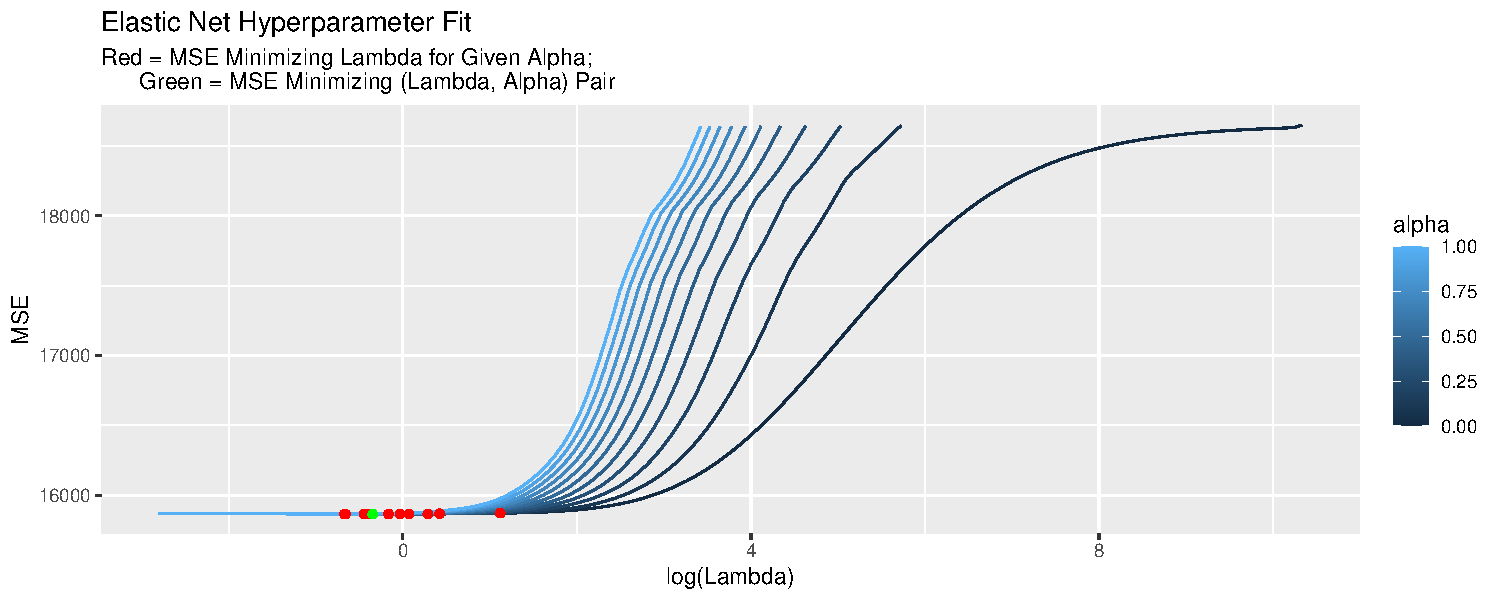
\includegraphics[width=5in,height=2in]{figure/unnamed-chunk-6-1} 

}



\begin{kframe}
\begin{alltt}
  \hlstd{glmOptim} \hlopt
    \hlkwd{xtable}\hlstd{(.,} \hlkwc{caption} \hlstd{=} \hlstr{'Optimal Hyperparameters'}\hlstd{)} \hlopt
    \hlkwd{print}\hlstd{(.)}
\end{alltt}
\end{kframe}% latex table generated in R 4.0.3 by xtable 1.8-4 package
% Mon Jan 11 15:11:15 2021
\begin{table}[!h]
\centering
\begingroup\footnotesize
\begin{tabular}{rrrll}
  \hline
alpha & lambda & mse & min\_lambda\_for\_given\_alpha & min\_overall \\ 
  \hline
0.60 & 0.71 & 15865.17 & TRUE & TRUE \\ 
   \hline
\end{tabular}
\endgroup
\caption{Optimal Hyperparameters} 
\end{table}


These hyperparameters are then used to estimate the coefficients, shown in the below table. Note that two coefficients have been shrunken to zero and effectively removed from the regression, indicating these coefficients had little predictive power.\\


\begin{kframe}
\begin{alltt}
  \hlstd{glmObj} \hlkwb{=}
    \hlstd{glmnet}\hlopt{::}\hlkwd{glmnet}\hlstd{(}
      \hlkwc{x} \hlstd{= trainDf} \hlopt \hlstd{dplyr}\hlopt{::}\hlkwd{select}\hlstd{(.,} \hlopt{-}\hlstd{time_sleeping)} \hlopt \hlkwd{as.matrix}\hlstd{(.),}
      \hlkwc{y} \hlstd{= trainDf} \hlopt \hlstd{dplyr}\hlopt{::}\hlkwd{select}\hlstd{(., time_sleeping)} \hlopt \hlkwd{as.matrix}\hlstd{(.),}
      \hlkwc{alpha} \hlstd{= glmOptim}\hlopt{$}\hlstd{alpha,}
      \hlkwc{lambda} \hlstd{= glmOptim}\hlopt{$}\hlstd{lambda}
    \hlstd{)}

  \hlstd{coefMat} \hlkwb{=} \hlstd{glmObj} \hlopt \hlkwd{coef}\hlstd{(.)} \hlopt \hlkwd{as.matrix}\hlstd{(.)}

  \hlstd{coefMat} \hlopt
    \hlkwd{as.data.frame}\hlstd{(.)} \hlopt
    \hlkwd{rownames_to_column}\hlstd{(.,} \hlkwc{var} \hlstd{=} \hlstr{'Covariate'}\hlstd{)} \hlopt
    \hlkwd{setNames}\hlstd{(.,} \hlkwd{c}\hlstd{(}\hlstr{'Covariate'}\hlstd{,} \hlstr{'Estimate'}\hlstd{))} \hlopt
    \hlkwd{xtable}\hlstd{(.,} \hlkwc{caption} \hlstd{=} \hlstr{'Elastic Net Estimates'}\hlstd{,} \hlkwc{digits} \hlstd{=} \hlnum{5}\hlstd{)} \hlopt
    \hlkwd{print}\hlstd{(.)}
\end{alltt}
\end{kframe}% latex table generated in R 4.0.3 by xtable 1.8-4 package
% Mon Jan 11 15:11:15 2021
\begin{table}[!h]
\centering
\begingroup\footnotesize
\begin{tabular}{lr}
  \hline
Covariate & Estimate \\ 
  \hline
(Intercept) & 729.06338 \\ 
  time\_insomnia & -0.49894 \\ 
  age & -0.60369 \\ 
  is\_male & -3.47788 \\ 
  is\_student & -4.48876 \\ 
  is\_employed & -20.12913 \\ 
  has\_children & 17.40865 \\ 
  number\_children & -4.81052 \\ 
  age\_youngest\_child & 0.00000 \\ 
  weekly\_earnings & -0.00055 \\ 
  hh\_size & -1.38152 \\ 
  spouse\_hours & -0.20265 \\ 
  hours\_working & -0.92708 \\ 
  time\_alone & -0.20383 \\ 
  time\_childcare & 0.00000 \\ 
  time\_family & -0.12707 \\ 
  time\_friends & -0.14868 \\ 
  time\_eldercare & -0.01909 \\ 
   \hline
\end{tabular}
\endgroup
\caption{Elastic Net Estimates} 
\end{table}

We then multiply the coefficient matrix by the test data matrix to get the predicted values of \texttt{time\_sleep}. Then we subtract these from the actual test data to get the residuals. Goodness-of-fit statistics are shown below.\\
\begin{kframe}
\begin{alltt}
  \hlcom{# OOS fitting}
  \hlstd{oosFit} \hlkwb{=}
    \hlstd{testDf} \hlopt
    \hlstd{dplyr}\hlopt{::}\hlkwd{select}\hlstd{(.,} \hlopt{-}\hlstd{time_sleeping)} \hlopt
    \hlstd{dplyr}\hlopt{::}\hlkwd{bind_cols}\hlstd{(}\hlkwc{constant} \hlstd{=} \hlnum{1}\hlstd{, .)} \hlopt
    \hlkwd{as.matrix}\hlstd{(.)} \hlopt
    \hlstd{\{.} \hlopt \hlstd{coefMat\}} \hlopt
    \hlkwd{as.data.frame}\hlstd{(.)} \hlopt
    \hlkwd{as_tibble}\hlstd{(.)} \hlopt
    \hlkwd{setNames}\hlstd{(.,} \hlstr{'yhat'}\hlstd{)}

  \hlcom{# Get residuals and goodness-of-fit statistics}
  \hlstd{gofDf} \hlkwb{=}
    \hlstd{oosFit} \hlopt
    \hlstd{dplyr}\hlopt{::}\hlkwd{bind_cols}\hlstd{(.,} \hlkwc{y} \hlstd{= testDf}\hlopt{$}\hlstd{time_sleeping)} \hlopt
    \hlstd{dplyr}\hlopt{::}\hlkwd{mutate}\hlstd{(.,} \hlkwc{resids} \hlstd{= y} \hlopt{-} \hlstd{yhat)} \hlopt
    \hlstd{dplyr}\hlopt{::}\hlkwd{summarize}\hlstd{(.,} \hlkwc{MAE} \hlstd{=} \hlkwd{mean}\hlstd{(}\hlkwd{abs}\hlstd{(resids)),} \hlkwc{SSE} \hlstd{=} \hlkwd{sum}\hlstd{(resids}\hlopt{^}\hlnum{2}\hlstd{),} \hlkwc{MSE} \hlstd{=} \hlkwd{mean}\hlstd{(resids}\hlopt{^}\hlnum{2}\hlstd{))}

  \hlstd{gofDf} \hlopt
    \hlkwd{xtable}\hlstd{(.,} \hlkwc{caption} \hlstd{=} \hlstr{'Elastic Net OOS Goodness-of-Fit'}\hlstd{)} \hlopt
    \hlkwd{print}\hlstd{(.)}
\end{alltt}
\end{kframe}% latex table generated in R 4.0.3 by xtable 1.8-4 package
% Mon Jan 11 15:11:15 2021
\begin{table}[!h]
\centering
\begingroup\footnotesize
\begin{tabular}{rrr}
  \hline
MAE & SSE & MSE \\ 
  \hline
93.20 & 70222973.69 & 14884.06 \\ 
   \hline
\end{tabular}
\endgroup
\caption{Elastic Net OOS Goodness-of-Fit} 
\end{table}

Finally, we run a typical OLS regression on the same training dataset. Coefficients are shown below.\\
\begin{kframe}
\begin{alltt}
  \hlkwd{lm}\hlstd{(time_sleeping} \hlopt{~} \hlstd{., sleepDf)} \hlopt
    \hlkwd{xtable}\hlstd{(.,} \hlkwc{caption} \hlstd{=} \hlstr{'OLS Regression Results'}\hlstd{)} \hlopt
    \hlkwd{print}\hlstd{(.,} \hlkwc{include.rownames} \hlstd{=} \hlnum{TRUE}\hlstd{)}
\end{alltt}
\end{kframe}% latex table generated in R 4.0.3 by xtable 1.8-4 package
% Mon Jan 11 15:11:15 2021
\begin{table}[!h]
\centering
\begingroup\footnotesize
\begin{tabular}{rrrrr}
  \hline
 & Estimate & Std. Error & t value & Pr($>$$|$t$|$) \\ 
  \hline
(Intercept) & 731.1363 & 8.1734 & 89.45 & 0.0000 \\ 
  time\_insomnia & -0.5490 & 0.0407 & -13.47 & 0.0000 \\ 
  age & -0.6415 & 0.0999 & -6.42 & 0.0000 \\ 
  is\_male & -1.4873 & 2.6397 & -0.56 & 0.5732 \\ 
  is\_student & -5.8462 & 6.7815 & -0.86 & 0.3887 \\ 
  is\_employed & -27.5152 & 4.7443 & -5.80 & 0.0000 \\ 
  has\_children & 4.4790 & 12.1576 & 0.37 & 0.7126 \\ 
  number\_children & -8.0169 & 2.3913 & -3.35 & 0.0008 \\ 
  age\_youngest\_child & 0.7858 & 0.3110 & 2.53 & 0.0115 \\ 
  weekly\_earnings & 0.0001 & 0.0002 & 0.39 & 0.6959 \\ 
  hh\_size & -1.0306 & 1.6631 & -0.62 & 0.5355 \\ 
  spouse\_hours & -0.2352 & 0.0684 & -3.44 & 0.0006 \\ 
  hours\_working & -0.8608 & 0.1014 & -8.49 & 0.0000 \\ 
  time\_alone & -0.1995 & 0.0061 & -32.49 & 0.0000 \\ 
  time\_childcare & 0.0059 & 0.0086 & 0.68 & 0.4946 \\ 
  time\_family & -0.1295 & 0.0071 & -18.19 & 0.0000 \\ 
  time\_friends & -0.1499 & 0.0112 & -13.34 & 0.0000 \\ 
  time\_eldercare & -0.0456 & 0.0198 & -2.31 & 0.0210 \\ 
   \hline
\end{tabular}
\endgroup
\caption{OLS Regression Results} 
\end{table}

We find the predicted values by using the OLS estimated coefficients on the test data matrix. Residuals are calculated and goodness-of-fit statistics are shown below.\\
\begin{kframe}
\begin{alltt}
  \hlcom{# Now compare to regular OLS}
  \hlstd{olsOosFit} \hlkwb{=}
    \hlstd{testDf} \hlopt
    \hlstd{dplyr}\hlopt{::}\hlkwd{select}\hlstd{(.,} \hlopt{-}\hlstd{time_sleeping)} \hlopt
    \hlstd{dplyr}\hlopt{::}\hlkwd{bind_cols}\hlstd{(}\hlkwc{constant} \hlstd{=} \hlnum{1}\hlstd{, .)} \hlopt
    \hlkwd{as.matrix}\hlstd{(.)} \hlopt
    \hlstd{\{.} \hlopt \hlkwd{coef}\hlstd{(}\hlkwd{lm}\hlstd{(time_sleeping} \hlopt{~} \hlstd{., sleepDf))\}} \hlopt
    \hlkwd{as.data.frame}\hlstd{(.)} \hlopt
    \hlkwd{as_tibble}\hlstd{(.)} \hlopt
    \hlkwd{setNames}\hlstd{(.,} \hlstr{'yhat'}\hlstd{)}

  \hlstd{olsGofDf} \hlkwb{=}
    \hlstd{olsOosFit} \hlopt
    \hlstd{dplyr}\hlopt{::}\hlkwd{bind_cols}\hlstd{(.,} \hlkwc{y} \hlstd{= testDf}\hlopt{$}\hlstd{time_sleeping)} \hlopt
    \hlstd{dplyr}\hlopt{::}\hlkwd{mutate}\hlstd{(.,} \hlkwc{resids} \hlstd{= y} \hlopt{-} \hlstd{yhat)} \hlopt
    \hlstd{dplyr}\hlopt{::}\hlkwd{summarize}\hlstd{(.,} \hlkwc{MAE} \hlstd{=} \hlkwd{mean}\hlstd{(}\hlkwd{abs}\hlstd{(resids)),} \hlkwc{SSE} \hlstd{=} \hlkwd{sum}\hlstd{(resids}\hlopt{^}\hlnum{2}\hlstd{),} \hlkwc{MSE} \hlstd{=} \hlkwd{mean}\hlstd{(resids}\hlopt{^}\hlnum{2}\hlstd{))}

  \hlstd{olsGofDf} \hlopt
    \hlkwd{xtable}\hlstd{(.,} \hlkwc{caption} \hlstd{=} \hlstr{'OLS OOS Goodness-of-Fit'}\hlstd{)} \hlopt
    \hlkwd{print}\hlstd{(.)}
\end{alltt}
\end{kframe}% latex table generated in R 4.0.3 by xtable 1.8-4 package
% Mon Jan 11 15:11:15 2021
\begin{table}[!h]
\centering
\begingroup\footnotesize
\begin{tabular}{rrr}
  \hline
MAE & SSE & MSE \\ 
  \hline
92.78 & 69608439.69 & 14753.80 \\ 
   \hline
\end{tabular}
\endgroup
\caption{OLS OOS Goodness-of-Fit} 
\end{table}


OLS ends up providing a better out-of-sample fit than the elastic net process. This is likely because in the OLS results, almost all the regression coefficients are significant, suggesting that they all have some predictive power on \texttt{time\_sleeping}. This implies that any shrinkage of covariates from the elastic net regularization process will have little positive effect on out-of-sample forecasting. This tells us that standard OLS may be a better choice than machine learning techniques when the covariates are intuitively and clearly relevant to the dependent variable.\\



\clearpage
\section{SVM Estimation}

\begin{kframe}
\begin{alltt}
  \hlcom{# Create dataset}
  \hlstd{sleepDf2} \hlkwb{=}
    \hlstd{sleepDf} \hlopt
    \hlstd{dplyr}\hlopt{::}\hlkwd{mutate}\hlstd{(.,} \hlkwc{has_insomnia} \hlstd{=} \hlkwd{ifelse}\hlstd{(time_insomnia} \hlopt{>} \hlnum{0}\hlstd{,} \hlnum{1}\hlstd{,} \hlnum{0}\hlstd{))} \hlopt
    \hlstd{dplyr}\hlopt{::}\hlkwd{mutate}\hlstd{(.,} \hlkwc{has_insomnia} \hlstd{=} \hlkwd{as.factor}\hlstd{(has_insomnia))} \hlopt
    \hlstd{dplyr}\hlopt{::}\hlkwd{select}\hlstd{(.,} \hlopt{-}\hlstd{time_insomnia)}

  \hlstd{trainDf} \hlkwb{=} \hlstd{sleepDf2[}\hlnum{1}\hlopt{:}\hlstd{(}\hlkwd{floor}\hlstd{(}\hlkwd{nrow}\hlstd{(sleepDf2)}\hlopt{/}\hlnum{2}\hlstd{)),]}
  \hlstd{testDf} \hlkwb{=} \hlstd{sleepDf2[}\hlkwd{floor}\hlstd{(}\hlkwd{nrow}\hlstd{(sleepDf2)}\hlopt{/}\hlnum{2} \hlopt{+} \hlnum{1}\hlstd{)}\hlopt{:}\hlstd{(}\hlkwd{nrow}\hlstd{(sleepDf2)),]}

  \hlkwd{set.seed}\hlstd{(}\hlnum{12345}\hlstd{)}
  \hlcom{# Tune hyperparameters of SVM}
  \hlstd{tuneRes} \hlkwb{=}
    \hlkwd{tune.svm}\hlstd{(}
      \hlstd{has_insomnia} \hlopt{~} \hlstd{.,} \hlkwc{data} \hlstd{= sleepDf2,} \hlkwc{kernel} \hlstd{=} \hlstr{'radial'}\hlstd{,}
      \hlkwc{type} \hlstd{=} \hlstr{'C-classification'}\hlstd{,} \hlkwc{cost} \hlstd{=} \hlnum{2}\hlopt{^}\hlstd{(}\hlnum{0}\hlopt{:}\hlnum{3}\hlstd{)}
      \hlstd{)}

  \hlstd{tuneRes2} \hlkwb{=}
    \hlkwd{tune.svm}\hlstd{(}
      \hlstd{has_insomnia} \hlopt{~} \hlstd{.,} \hlkwc{data} \hlstd{= sleepDf2,}
      \hlkwc{kernel} \hlstd{=} \hlstr{'linear'}\hlstd{,} \hlkwc{type} \hlstd{=} \hlstr{'C-classification'}\hlstd{,} \hlkwc{cost} \hlstd{=} \hlnum{2}\hlopt{^}\hlstd{(}\hlnum{0}\hlopt{:}\hlnum{3}\hlstd{)}
      \hlstd{)}

  \hlcom{# Do OOS testing of SVM}
  \hlstd{svmFit} \hlkwb{=}
    \hlstd{tuneRes}\hlopt{$}\hlstd{best.model} \hlopt
    \hlkwd{predict}\hlstd{(.,} \hlkwc{newdata} \hlstd{= testDf} \hlopt \hlstd{dplyr}\hlopt{::}\hlkwd{select}\hlstd{(.,} \hlopt{-}\hlstd{has_insomnia))}

  \hlstd{svmGofDf} \hlkwb{=}
    \hlkwd{tibble}\hlstd{(}\hlkwc{yhat} \hlstd{= svmFit,} \hlkwc{y} \hlstd{= testDf}\hlopt{$}\hlstd{has_insomnia)} \hlopt
    \hlstd{dplyr}\hlopt{::}\hlkwd{mutate}\hlstd{(.,} \hlkwc{resids} \hlstd{=} \hlkwd{as.numeric}\hlstd{(y)} \hlopt{-} \hlkwd{as.numeric}\hlstd{(yhat))} \hlopt
    \hlstd{dplyr}\hlopt{::}\hlkwd{summarize}\hlstd{(.,} \hlkwc{MAE} \hlstd{=} \hlkwd{mean}\hlstd{(}\hlkwd{abs}\hlstd{(resids)),} \hlkwc{SSE} \hlstd{=} \hlkwd{sum}\hlstd{(resids}\hlopt{^}\hlnum{2}\hlstd{),} \hlkwc{MSE} \hlstd{=} \hlkwd{mean}\hlstd{(resids}\hlopt{^}\hlnum{2}\hlstd{))}

  \hlcom{# Run regular logit model and do OOS testing}
  \hlstd{glmGofDf} \hlkwb{=}
    \hlkwd{glm}\hlstd{(has_insomnia} \hlopt{~} \hlstd{.,} \hlkwc{data} \hlstd{= trainDf,} \hlkwc{family} \hlstd{=} \hlstr{'binomial'}\hlstd{)} \hlopt
    \hlkwd{predict}\hlstd{(}
      \hlstd{.,}
      \hlkwc{newdata} \hlstd{= testDf} \hlopt \hlstd{dplyr}\hlopt{::}\hlkwd{select}\hlstd{(.,} \hlopt{-}\hlstd{has_insomnia),}
      \hlkwc{type} \hlstd{=} \hlstr{'response'}
      \hlstd{)} \hlopt
    \hlkwd{tibble}\hlstd{(}\hlkwc{yhat} \hlstd{= .,} \hlkwc{y} \hlstd{= testDf}\hlopt{$}\hlstd{has_insomnia)} \hlopt
    \hlstd{dplyr}\hlopt{::}\hlkwd{mutate}\hlstd{(.,} \hlkwc{resids} \hlstd{=} \hlkwd{as.numeric}\hlstd{(y)} \hlopt{-} \hlkwd{as.numeric}\hlstd{(yhat))} \hlopt
    \hlstd{dplyr}\hlopt{::}\hlkwd{summarize}\hlstd{(.,} \hlkwc{MAE} \hlstd{=} \hlkwd{mean}\hlstd{(}\hlkwd{abs}\hlstd{(resids)),} \hlkwc{SSE} \hlstd{=} \hlkwd{sum}\hlstd{(resids}\hlopt{^}\hlnum{2}\hlstd{),} \hlkwc{MSE} \hlstd{=} \hlkwd{mean}\hlstd{(resids}\hlopt{^}\hlnum{2}\hlstd{))}
\end{alltt}
\end{kframe}
We now alter the dataset used previously to create a new dependent variable, \texttt{has\_insomnia}, a binary variable indicating whether the individual experienced any minutes of insomnia over the past week. Our independent variables are now \textit{time\_sleeping, age, is\_male, is\_student, is\_employed, has\_children, number\_children, age\_youngest\_child, weekly\_earnings, hh\_size, spouse\_hours, hours\_working, time\_alone, time\_childcare, time\_family, time\_friends, time\_eldercare}.\\

As before, we break up the dataset into a testing and training dataset. We run two alternative kernels, radial and linear, and use the \texttt{tune} function to perform a grid search over the cost functions $2^0, 2^1, \dots, 2^5$. We find that the lowest error is provided by the linear kernel with cost function 1.\\

We fit this SVM model to the test dataset and derive the following out-of-sample goodness-of-fit statistics for the residuals.\\
\begin{kframe}
\begin{alltt}
  \hlstd{svmGofDf} \hlopt
    \hlkwd{xtable}\hlstd{(.,} \hlkwc{caption} \hlstd{=} \hlstr{'SVM Goodness-of-Fit'}\hlstd{)} \hlopt
    \hlkwd{print}\hlstd{(.)}
\end{alltt}
\end{kframe}% latex table generated in R 4.0.3 by xtable 1.8-4 package
% Mon Jan 11 15:16:31 2021
\begin{table}[!h]
\centering
\begingroup\footnotesize
\begin{tabular}{rrr}
  \hline
MAE & SSE & MSE \\ 
  \hline
0.08 & 369.00 & 0.08 \\ 
   \hline
\end{tabular}
\endgroup
\caption{SVM Goodness-of-Fit} 
\end{table}


To benchmark the SVM model, we fit a standard logit model as well and derive the coefficient estimates below.\\
\begin{kframe}
\begin{alltt}
  \hlkwd{glm}\hlstd{(has_insomnia} \hlopt{~} \hlstd{.,} \hlkwc{data} \hlstd{= trainDf,} \hlkwc{family} \hlstd{=} \hlstr{'binomial'}\hlstd{)} \hlopt
    \hlkwd{xtable}\hlstd{(.,} \hlkwc{caption} \hlstd{=} \hlstr{'Logit Model Fit'}\hlstd{)} \hlopt
    \hlkwd{print}\hlstd{(.,} \hlkwc{include.rownames} \hlstd{=} \hlnum{TRUE}\hlstd{)}
\end{alltt}
\end{kframe}% latex table generated in R 4.0.3 by xtable 1.8-4 package
% Mon Jan 11 15:16:31 2021
\begin{table}[!h]
\centering
\begingroup\footnotesize
\begin{tabular}{rrrrr}
  \hline
 & Estimate & Std. Error & z value & Pr($>$$|$z$|$) \\ 
  \hline
(Intercept) & -0.4326 & 0.4696 & -0.92 & 0.3570 \\ 
  time\_sleeping & -0.0021 & 0.0004 & -4.85 & 0.0000 \\ 
  age & 0.0022 & 0.0043 & 0.50 & 0.6149 \\ 
  is\_male & -0.3983 & 0.1173 & -3.39 & 0.0007 \\ 
  is\_student & -0.0694 & 0.2987 & -0.23 & 0.8162 \\ 
  is\_employed & -0.5222 & 0.2116 & -2.47 & 0.0136 \\ 
  has\_children & -1.1782 & 1.0181 & -1.16 & 0.2472 \\ 
  number\_children & -0.0777 & 0.1056 & -0.74 & 0.4618 \\ 
  age\_youngest\_child & -0.0035 & 0.0143 & -0.25 & 0.8055 \\ 
  weekly\_earnings & -0.0000 & 0.0000 & -0.93 & 0.3546 \\ 
  hh\_size & 0.0840 & 0.0694 & 1.21 & 0.2261 \\ 
  spouse\_hours & 0.0024 & 0.0030 & 0.81 & 0.4186 \\ 
  hours\_working & -0.0034 & 0.0047 & -0.71 & 0.4750 \\ 
  time\_alone & -0.0007 & 0.0003 & -2.44 & 0.0148 \\ 
  time\_childcare & -0.0002 & 0.0004 & -0.54 & 0.5903 \\ 
  time\_family & -0.0012 & 0.0003 & -3.83 & 0.0001 \\ 
  time\_friends & -0.0021 & 0.0007 & -3.23 & 0.0012 \\ 
  time\_eldercare & -0.0016 & 0.0013 & -1.23 & 0.2171 \\ 
   \hline
\end{tabular}
\endgroup
\caption{Logit Model Fit} 
\end{table}


\begin{kframe}
\begin{alltt}
  \hlstd{glmGofDf} \hlopt
    \hlkwd{xtable}\hlstd{(.,} \hlkwc{caption} \hlstd{=} \hlstr{'Logit Model Goodness-of-Fit'}\hlstd{)} \hlopt
    \hlkwd{print}\hlstd{(.)}
\end{alltt}
\end{kframe}% latex table generated in R 4.0.3 by xtable 1.8-4 package
% Mon Jan 11 15:16:31 2021
\begin{table}[!h]
\centering
\begingroup\footnotesize
\begin{tabular}{rrr}
  \hline
MAE & SSE & MSE \\ 
  \hline
1.00 & 5058.33 & 1.07 \\ 
   \hline
\end{tabular}
\endgroup
\caption{Logit Model Goodness-of-Fit} 
\end{table}


Comparison of the out-of-sample testing results between the models suggests that SVM performs the better fit. This is likely because the data is high-dimensional but we have relatively few observations; moreover the independent variables likely have a nonlinear relationship with the dependent variable (e.g. demographic covariates like age tend to have nonlinear, nonmonotonic effects on a person's likelihood of having insomnia).




\end{document}
